% ==============================================================================
\chapter{CLIC: the Compact LInear Collider}
\label{ch:CLIC}
% ============================================================================== 

The energy loss due to the synchrotron radiation in a circular
accelerator limits the center-of-mass energy $\sqrt{s}$ reached by
electron beams. The energy loss is inversely proportional to the
bending radius of the accelerator and the particle mass. The proposed
Compact Linear Collider
(CLIC)~\cite{Aicheler:1500095,Linssen:1425915}, as a future linear
particle collider for electrons (e$^-$) and positrons (e$^+$), can
avoid synchrotron radiation losses and attain higher center-of-mass
energies than the Large Electron-Positron Collider (LEP).

Today, the Large Hadron Collider (LHC) is the largest particle
accelerator being able to collide two opposing particle beams of
protons with a center-of-mass energy up to $13\,\tev$. So far, the
main result of the LHC is the observation of the Higgs boson and the
determination of its mass in 2012. However, the experiments at the LHC
can not fully answer the questions on the nature of this particle. In
the post-LHC era, CLIC will allow to determine the properties of the
Higgs boson with a very high precision. CLIC can measure collisions
with center-of-mass energies from $380\,\gev$ up to $3\,\tev$.

In this chapter, we will briefly discuss the standard model of
particle physics and attempt to understand how CLIC can determine more
precisely the properties of the Higgs boson. Subsequently the CLIC
detector and its components are described. The focus is put on the
vertex detector, its requirements and its flavour-tagging performance.

\section{Physics potential at CLIC} 

In particle physics, the Standard Model (SM) is a theoretical
framework that describes how the interaction between elementary
particles is governed by four fundamental forces. This theory,
developed in the early 1970s, explains most of the experimental
results.

According to the Standard Model, matter is made of elementary
particles which can be regrouped into three basic kinds: quarks,
leptons and gauge bosons as shown in~\cref{fig:standardmodel}.

\begin{figure}[htbp]
  \centering
  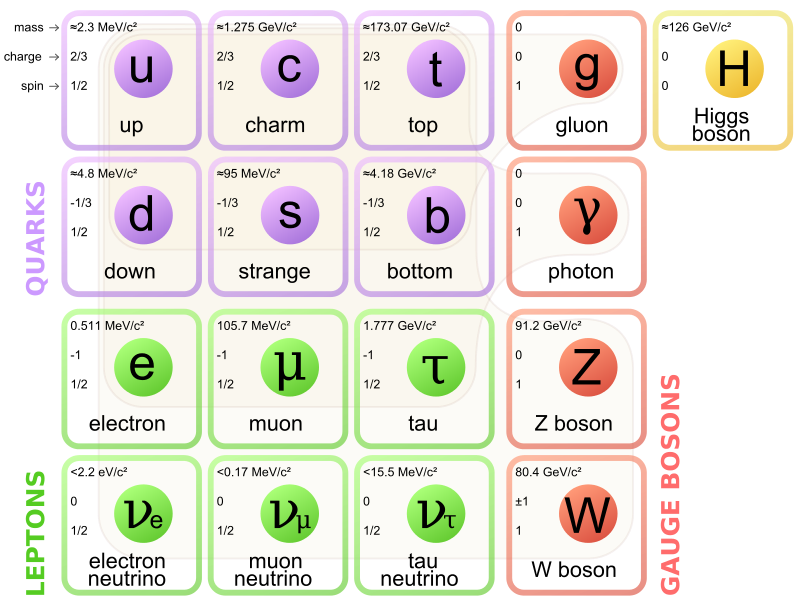
\includegraphics[width=0.7\textwidth]{figures/CLIC/StandardModel.png}
  \caption{The building blocks of matter according to the Standard
    Model~\cite{wikipediaParticles}.}
  \label{fig:standardmodel}
\end{figure}

Today, the Standard Model is the best theory describing the subatomic
world. However, it does not answer questions like the nature of dark
matter. This theory also predicts the existence of the Higgs boson
which gives the mass to all particles. It was experimentally observed
in 2012 by the LHC experiments.

The weak and the electromagnetic forces are closely related to each
other and can be unified as the \begin{it}electroweak\end{it} force
and the equations describing the unification predict the
force-carrying particles (the photon, the W and Z bosons). The only
problem is that all the force-carrying particles are described as
being massless which is true for the photon, but the W and Z bosons
have a mass about 100 times larger than that of the proton. To solve
this problem, the Brout-Englert-Higgs mechanism was introduced which
suggests that the Higgs boson gives the mass to the W and Z boson by
interaction with a Higgs field.

The Higgs particle can be produced in a particle collider by the
collision between highly energetic particles. Heavy particles, like
the Higgs boson, are occasionally produced and then detected by a
particle detector. The Standard Model predicts different mechanisms to
produce the Higgs boson and the probability to produce it is very
small. For example, in LHC only 1 Higgs boson is produced per 10
billion collisions.

An electron-positron collider allows to perform precision measurements
by colliding beams made of elementary particles. In fact, with
elementary particles, the center-of-mass energy and the polarisation
of the colliding particles can be selected precisely. Unlike
proton-proton collisions at the LHC experiments, there is no
underlying event from proton remnants.


CLIC is foreseen to be built and operated in three stages with
center-of-mass energies of $380\,\gev$, $1.5\,\tev$ and $3\,\tev$ as
shown in \cref{fig:CLICstaging}~\cite{Felzmann:2157041}. The site
studies have shown that CLIC could be placed near CERN
underground. For each stage, to increase the center-of-mass energy,
more accelerating modules will be needed, making the accelerator
longer. The site length for $3\,\tev$ will be 50~km.

\begin{figure}[htbp]
  \centering
  \includegraphics[width=0.7\textwidth]{figures/CLIC/staging.pdf}
  \caption{The three implementation stages of CLIC near CERN with
    center-of-mass energies of $380\,\gev$, $1.5\,\tev$ and
    $3\,\tev$~\cite{Felzmann:2157041}.}
  \label{fig:CLICstaging}
\end{figure}

The different energy stages at CLIC allow for maximising the
luminosity performance and physics potential for high precision
measurements of Standard Model physics (e.g. Higgs, top) as well as
new physics potentially discovered at the $13\,\tev$ LHC.

The first energy stage allows for studying the Standard Model Higgs
physics and top-quark physics with the possibility to perform a t\={t}
threshold scan. The second energy stage provides direct sensitivity to
many physics beyond the SM (BSM) models. With higher Higgs statistics,
rare decays such as t\={t}H and double Higgs productions can be
measured. Finally the third energy stage provides the best sensitivity
to new physics, the double-Higgs production allowing for improving the
measurements of the Higgs self-coupling and HHWW quartic
coupling. \cref{fig:HiggsProductionMechanisms} shows different
mechanisms to produce the Higgs boson at CLIC.
\begin{figure}[htbp]
  \centering
  \includegraphics[page=43, trim=30mm 235mm 10mm 30mm, clip, width=0.7\textwidth]{figures/CLIC/clicCDR.pdf}
  \caption{Standard Model Higgs boson production mechanisms at
    CLIC~\cite{Linssen:1425915}.}
  \label{fig:HiggsProductionMechanisms}
\end{figure}

The cross sections to produce a Higgs with a mass of $M_H = 126\,\gev$
as a function of the center-of-mass energy $\sqrt{s}$ is given in
\cref{fig:corssSectionH125}. Below $\sqrt{s}$ of $\sim500\,\gev$, the
HZ mechanism is dominant. For higher energies, the
H$\nu_{e}\bar{\nu_{e}}$ mechanism dominates.

\begin{figure}[htbp]
  \centering
  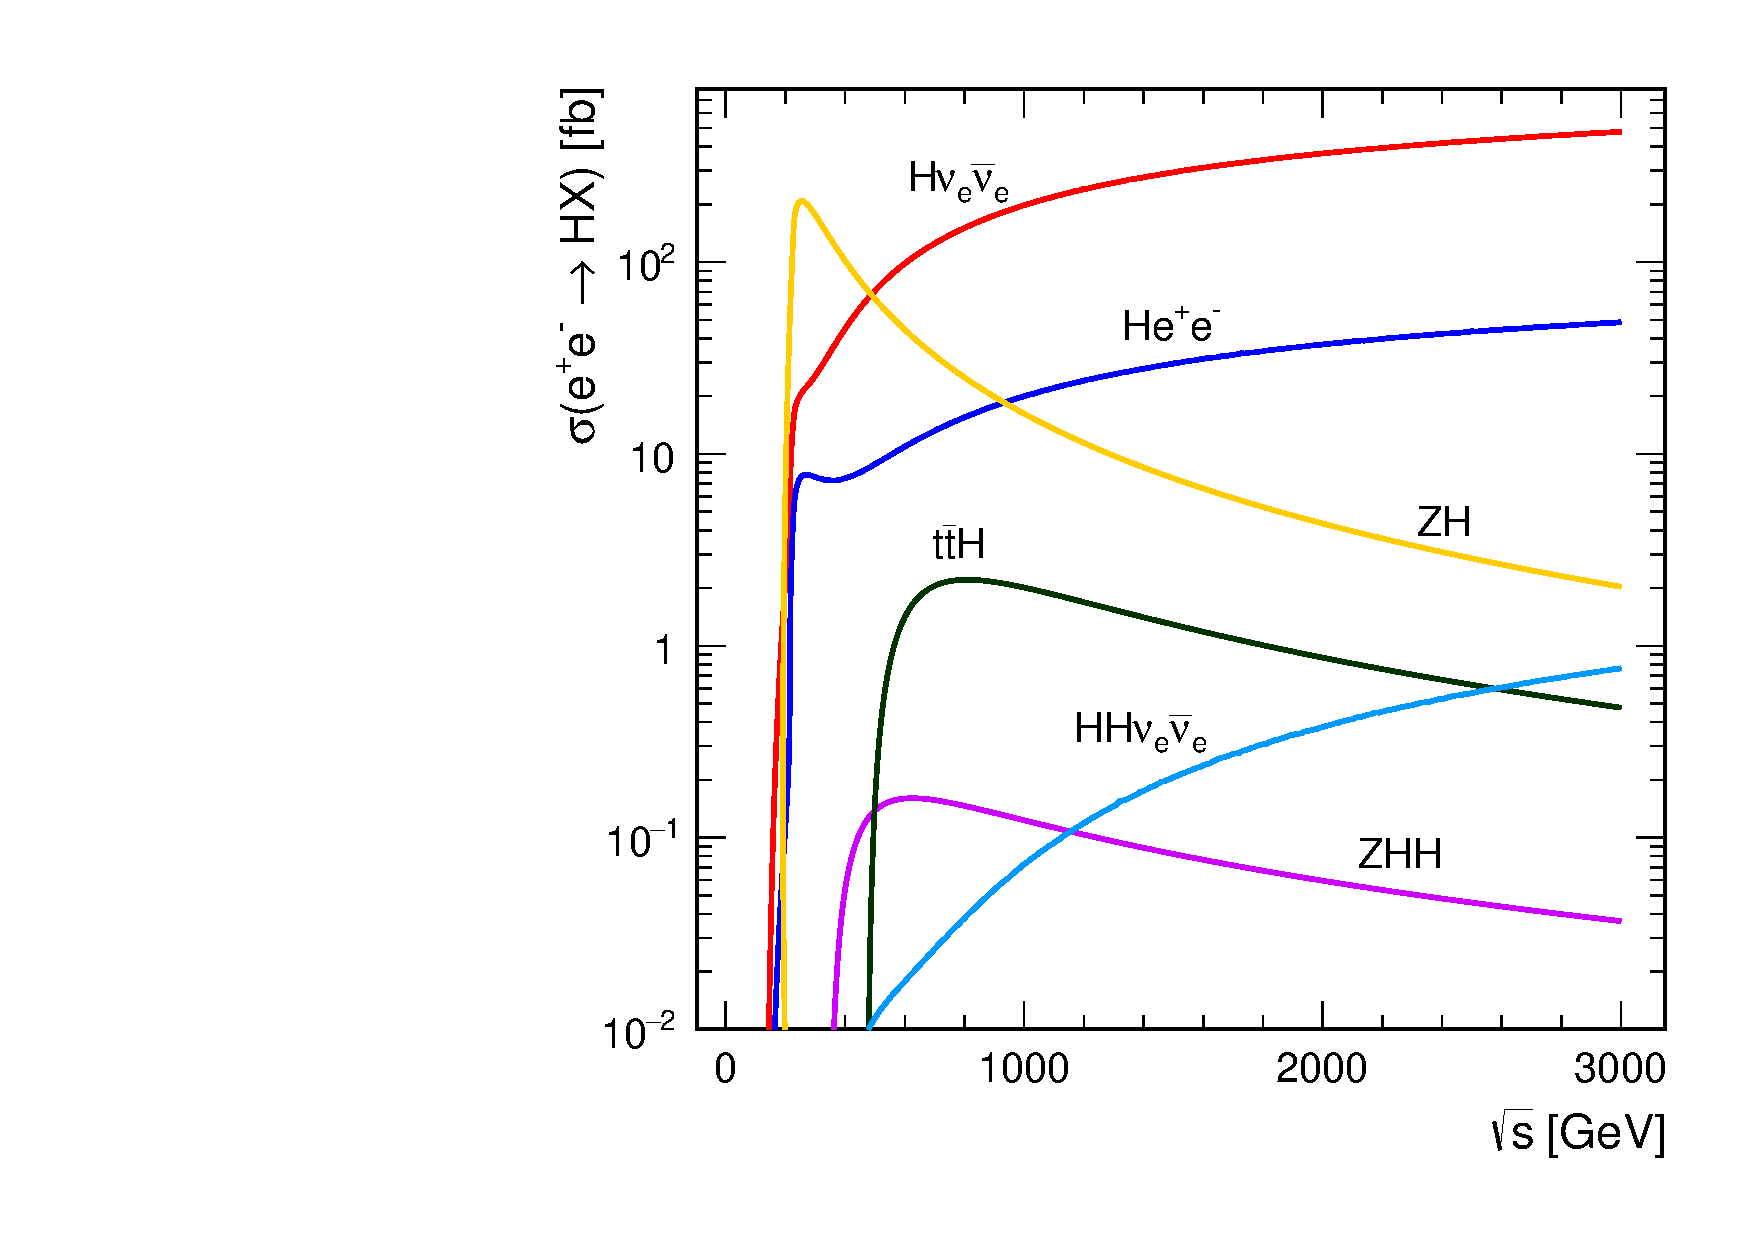
\includegraphics[width=0.5\textwidth]{figures/CLIC/xsec_vs_cme.pdf}
  \caption{Cross sections for the main Higgs production mechanisms for
    a $M_H~=~126\,\gev$ Higgs boson as a function of the e$^+$e$^-$
    center-of-mass energy in a lepton collider. These values
    correspond to unpolarised beams and the effect of beamstrahlung is
    not included~\cite{Felzmann:2157041}.}
  \label{fig:corssSectionH125}
\end{figure}


The CLIC accelerator uses copper cavities at room
temperature. Klystrons connected to the cavities provide the RF power
used by the acceleration cavities. The klystrons are not directly used
to accelerate the main beam at CLIC since a large number of them would
be needed and their efficiency would be too low. A two-beam
acceleration scheme is used to reach the nominal collision energy. A
drive beam with a low energy of $2.4\,\gev$ and a high current of
100~A is used to transfer the energy of the klystrons to the main beam
which has a lower current and higher energy. The drive beam is
decelerated over a distance of 878~m and the extracted energy is
provided to the main beam with a series of Power Extraction and
Transfer Systems (PETSs).

The schematic layout of the CLIC accelerator complex at
$\sqrt{s}=3\,\tev$ is shown in \cref{fig:CLIC_accelerator}. The
electron and positron beams are accelerated on a linear trajectory and
collide in the central region (in the interaction point), where the
CLIC detector is placed. At this stage, each linac is fed by a
drive-beam generation complex.

\begin{figure}[htbp]
  \centering
  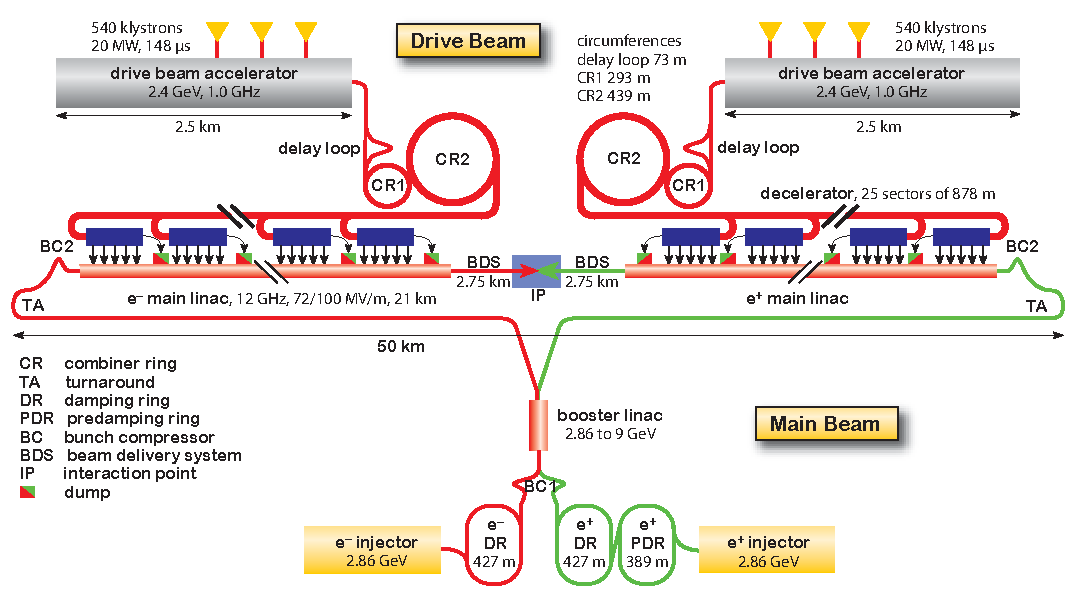
\includegraphics[width=\textwidth]{figures/CLIC/CLIC-layout2015pub.pdf}
  \caption{Schematic layout of the CLIC accelerator complex at
    $\sqrt{s}=3\,\tev$. At this stage, each linac is fed by a
    drive-beam generation complex~\cite{Felzmann:2157041}.}
  \label{fig:CLIC_accelerator}
\end{figure}


\section{Requirements for the CLIC vertex-detector}
\label{sec:VXD_requirements}

A detector concept covering the CLIC physics potential is under
development in simulations as shown in
\cref{fig:CLIC_detector_concept}. The physics goals set requirements
on the detector design.

\begin{figure}[htbp]
  \centering
  \begin{tikzpicture}
    \node[anchor=south west,inner sep=0] (image) at
    (0,0){\includegraphics[width=0.62\textwidth]{figures/CLIC/CLICdp_Top_view_HD_temp.pdf}};
    \begin{scope}[x={(image.south east)},y={(image.north west)}]
      %% \draw[help lines,xstep=.1,ystep=.1] (0, 0) grid (1,1);
      %% \foreach \x in {0,1,...,9} { \node [anchor=north] at (\x/10,0) {0.\x}; }
      %% \foreach \y in {0,1,...,9} { \node [anchor=east] at (0,\y/10)
      %% {0.\y}; }
      \node[draw, text width=2cm] at (-0.2, 0.9) {Ultra low-mass vertex detector};
      \draw[->,line width=1pt, color=black](-0.02, 0.9) -- (0.5, 0.5);

      \node[draw, text width=2cm] at (-0.2, 0.7) {Main tracker, silicon based};
      \draw[->,line width=1pt, color=black](-0.02, 0.7) -- (0.35, 0.55);

      \node[draw, text width=2cm] at (-0.2, 0.5) {Forward region with LumiCal \& BeamCal};
      \draw[->,line width=1pt, color=black](-0.02, 0.45) -- (0.25, 0.49);

      \node[draw, text width=2cm] at (-0.2, 0.2) {Fine grained calorimetry used in Particle Flow (PFA)};
      \draw[->,line width=1pt, color=black](-0.02, 0.2) -- (0.3, 0.3);

      \node[draw, text width=2cm] at (1.15, 0.15) {Return yoke (Fe) with detectors for muon ID};
      \draw[->,line width=1pt, color=black](1, 0.1) -- (0.8, 0.1);

      \node[draw, text width=2cm] at (1.15, 0.5) {Solenoid magnet: B=4~T};
      \draw[->,line width=1pt, color=black](1, 0.45) -- (0.7, 0.21);
      

      \node[color=black] at (0.5, 0.05) {11.4~m};
      \draw[<->,line width=1pt, color=black](0.03, 0.02) -- (0.97, 0.02);
      
    \end{scope}
  \end{tikzpicture} 
  \caption{Schematic layout of the CLIC detector concept.}
  \label{fig:CLIC_detector_concept}
\end{figure}

A broad detector R\&D program at CLIC is addressing the challenging
experimental conditions and the demands for precision physics. This
thesis focuses on the vertex-detector R\&D.

The main goal of the CLIC vertex detector is the efficient tagging of
heavy quarks through the precise measurement of the displaced
vertices. To achieve this goal, Monte Carlo simulations have shown
that a high-momentum term in the transverse impact-parameter
resolution of $a\approx5\,\micron$ and a multiple-scattering term of
$b\approx15\,\micron$ are needed using the canonical parametrisation:

\begin{equation}
 \sigma(d_0)=\sqrt{a^2+b^2 \cdot\gev^2/(p^2 \text{sin}^3\theta)} \; ,
  \label{eq:canonicalParam}
\end{equation}

where $p$ is the momentum of the particle and $\theta$ is the polar
angle with respect to the beam axis.

To meet these requirements, a multi-layer barrel and endcap pixel
detectors with an inner radius of $\approx$30~mm with a geometrical
coverage extending down to low polar angles
($\theta_{min}\approx8^{\circ}$) is needed. For the beam-pipe and for
each of the detection layers a material budget of $\approx0.2\%$ of a
radiation length (X\textsubscript{0}) is considered. Sensors with a
single-point resolution of $\approx3\,\micron$ operating in a magnetic
field of 4~T are required.

In the innermost layers, an occupancy of $\approx3\%$ due to the
beam-induced backgrounds is expected~\cite{Dannheim:1443516}. To
separate these backgrounds from physics events, a time slicing of the
hits with an accuracy of $\approx10$~ns is required.

In comparison to the current pixel detectors in the LHC experiments,
the exposure to radiation of the CLIC vertex detector is moderate. For
the inner-detector layers a total $1\,\mev$ neutron-equivalent fluence
of less than $10^{11}$~neq/cm\textsuperscript{2}/year and a total
ionising dose of less than 1~kGy are expected~\cite{Dannheim:1443516}.

The aim of the R\&D is to achieve the required single-point resolution
with pixels of size $\approx25\,\micron\times25\,\micron$ with
$50\,\micron$ thick sensors coupled to $50\,\micron$ thick analogue
readout ASICs. The constraint on the material budget implies no active
cooling elements can be placed inside the vertex detector. To limit
the maximum power dissipation of the readout electronics to
$\approx50~\text{mW/cm}^2$ forced air-flow cooling and power pulsing
(i.e. turning off most components on the readout chips during the
20~ms gaps between bunch trains) are foreseen.

\section{Flavour-tagging performance at CLIC}
\label{sec:flavourTagging}

The precision physics measurements require excellent flavour-tagging
performance of the CLIC vertex detector. The flavour-tagging
performance is studied in simulations. The multi-variate LCFIPlus
flavour-tagging package~\cite{website:LCFIPlus} is used to assign each
jet category with a beauty (b) and charm (c) probability. The fake
rates of recognising the charm and beauty jets from each other and
from light flavour (LF) jets are being investigated.

The detector models in simulation consider the single-point resolution
of the sensors ($\sim3\,\micron$), constraints from the mechanical
support and the cooling system~\cite{AlipourTehrani:1742993}.

As illustrated in Figure~\ref{fig:cooling}, a spiral arrangement for
the modules in the endcap regions can be used instead of disks,
allowing the air to flow through the vertex detector. The physics
performance of the geometries described in Table~\ref{tab:geometries}
and illustrated in Figure~\ref{fig:geometries} have been studied in
simulations.

\begin{table}[htbp]
  \caption{Vertex detector geometries implemented in simulations.}
  \begin{center}
    \begin{tabular}{ l c c c }
      \hline
      Geometry & Barrel layers & Endcap layers & Material budget \\ \hline \hline
      \emph{spirals} (Figure~\ref{fig:SpiralsGeometry}) & 5 single-sided & 4 single-sided & $0.1\%X_{0}$ per single-sided layer  \\ %\hline 
      \emph{double\_spirals} (Figure~\ref{fig:doubleLayer}) & 3 double-sided & 3 double-sided & $0.2\%X_{0}$ per double-sided layer  \\ %\hline
      \emph{double\_spirals\_v2} & 3 double-sided & 3 double-sided & $0.4\%X_{0}$ per double-sided layer  \\ \hline  
    \end{tabular}
  \end{center}
  \label{tab:geometries}
\end{table}


\begin{figure}[htbp]
  \begin{subfigure}[b]{0.33\textwidth}
    \centering
    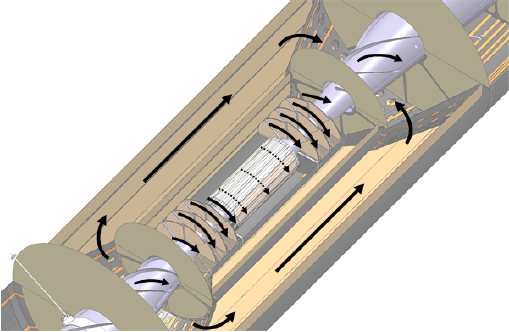
\includegraphics[width=\textwidth]{figures/CLIC/Cooling.png}  
    \caption{}
    \label{fig:cooling}
  \end{subfigure}~
  \begin{subfigure}[b]{0.33\textwidth}
    \centering
    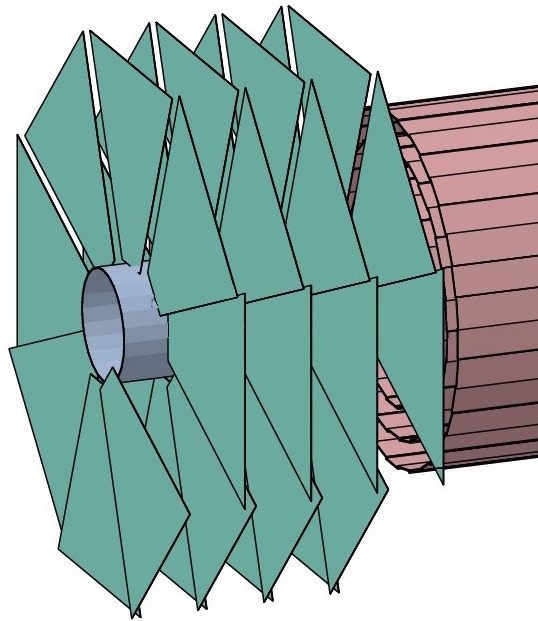
\includegraphics[width=0.65\textwidth]{figures/CLIC/single_spiral.jpg}
    \caption{}
    \label{fig:SpiralsGeometry}
  \end{subfigure}~
  \begin{subfigure}[b]{0.25\textwidth}
    \centering
    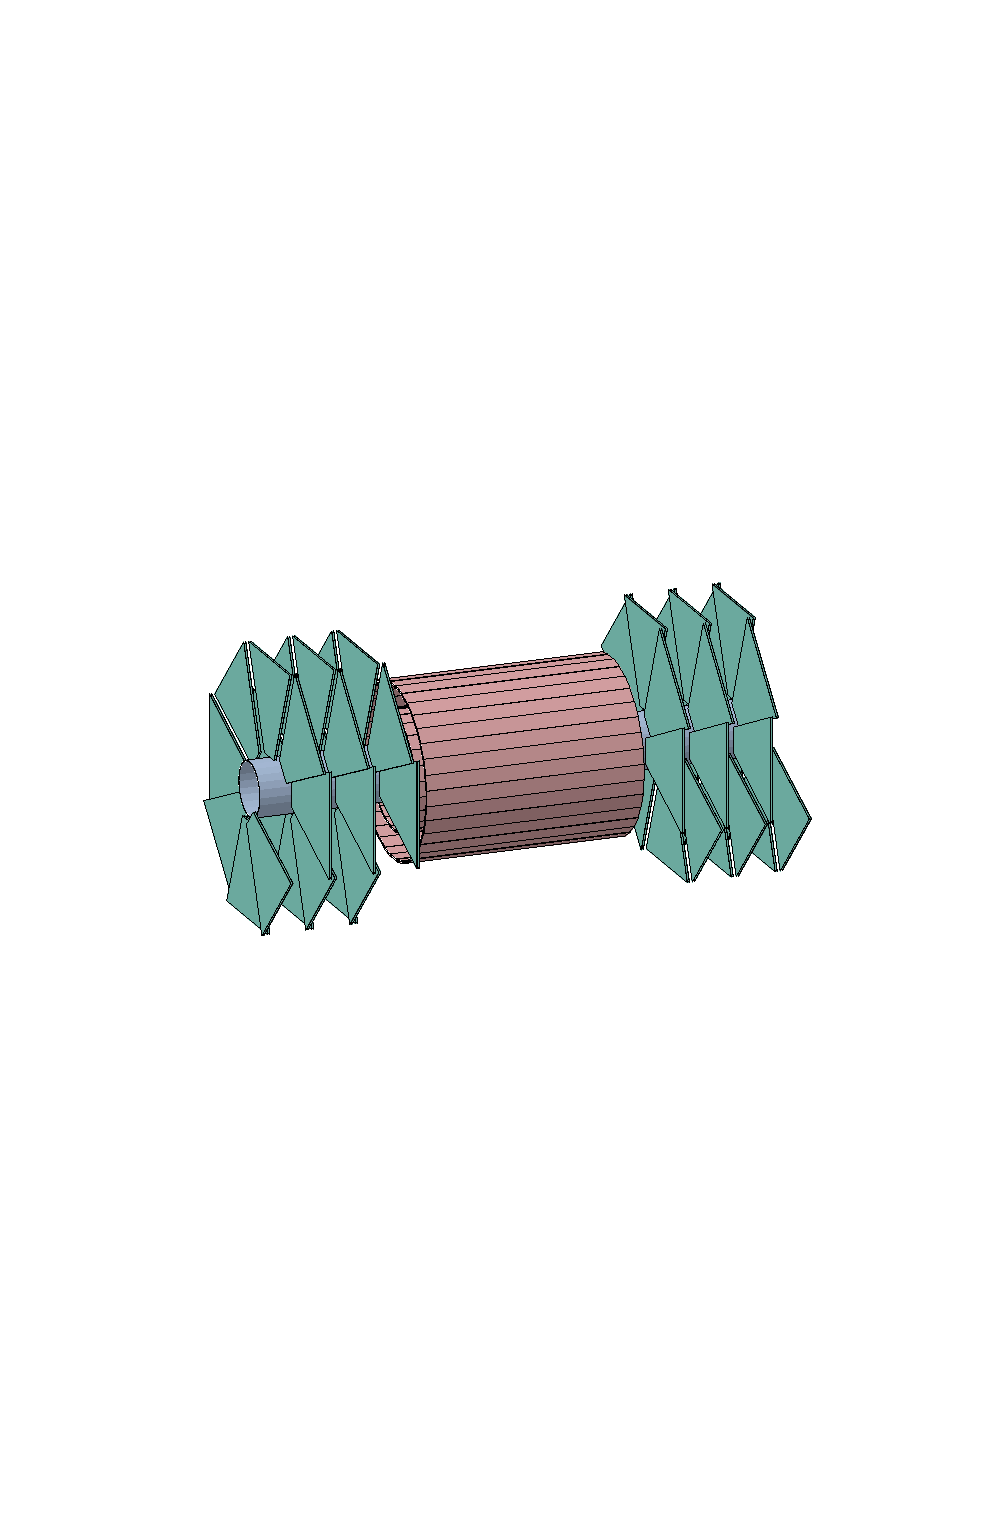
\includegraphics[trim = 32mm 98mm 85mm 106mm, clip, width=0.65\textwidth]{figures/CLIC/double_spiral.pdf} \\
    
\includegraphics[width=1.5\textwidth]{figures/CLIC/double_layer_module.png} 
    \caption{}
    \label{fig:doubleLayer}
  \end{subfigure}
  \caption{(a)~Sketch showing the airflow cooling strategy within the
    vertex detector~\cite{DuarteRamos:1572989}. (b)~Schematic view of
    the vertex detector for the \emph{spirals} geometry. (c)~Schematic
    view of the vertex detector for the
    \emph{double\_spirals(\_v2)}. In the \textsc{GEANT4}
    simulations~\cite{Agostinelli:2002hh}, a double-sided layer is
    implemented as two silicon sensors on top of each other with an
    overall thickness of \SI{2}{\milli\meter}.}
  \label{fig:geometries}
\end{figure}

The performance of the flavour tagging depends on the jet energy and
polar angle: dijet events with different center-of-mass energies,
$\sqrt{s}$, having polar angles of $10^{\circ} \leq \theta \leq
90^{\circ}$ with a uniform distribution in $\phi$ angles are
considered. Initial state radiation (ISR) and beamstrahlung (BS) were
switched off during the event generation and hence the final-state
quarks are in a back-to-back configuration. For each jet flavour,
energy and angle, 80000 events are used for the following processes:
e$^+$e$^-$ $\rightarrow$ b\={b}, c\={c}, u\={u}, d\={d}, s\={s}. The
boosted decision trees (BDTs) are trained using 50\% of the generated
events and the other 50\% are used for testing the performance of the
flavour tagging.

The flavour-tagging performance for the above-mentioned geometries is
summarised in \cref{fig:performance} where the fake rate of
recognising charm and light flavour jets as beauty jets is
plotted versus the b-tag efficiency.

The \emph{spirals} and \emph{disks} have a similar flavour-tagging
performance except for jets at $\theta=40^{\circ}$ (see
Figure~\ref{fig:spiral_disks}), which corresponds to the transition
between the vertex endcaps and the barrel region, where the
beauty-tagging performance is up to $20\%$ worse using the
\emph{spirals} geometry (compared to disks). With the spiral
configuration, the number of sensitive layers becomes dependent on the
azimuthal angle $\phi$ and fewer layers can be hit in certain ranges
of $\phi$. The performance of the \emph{spirals} and the
\emph{double\_spirals} is very similar as shown in
Figure~\ref{fig:spiral_doubleSpirals}.  The \emph{double\_spirals\_v2}
geometry is a more realistic version of the \emph{double\_spirals}
geometry, taking into account the material used for the mechanical
support of the sensors and also for the cables. As shown in
Figure~\ref{fig:doubleSpirals_doubleSpirals}, the misidentification
probability increases by $\sim$35\% due to the increased material.


\begin{figure}[htbp]
  \begin{subfigure}[b]{0.33\textwidth}
    \centering
    \begin{tikzpicture}
      \node[anchor=south west, inner sep=0] (image) at (0,0){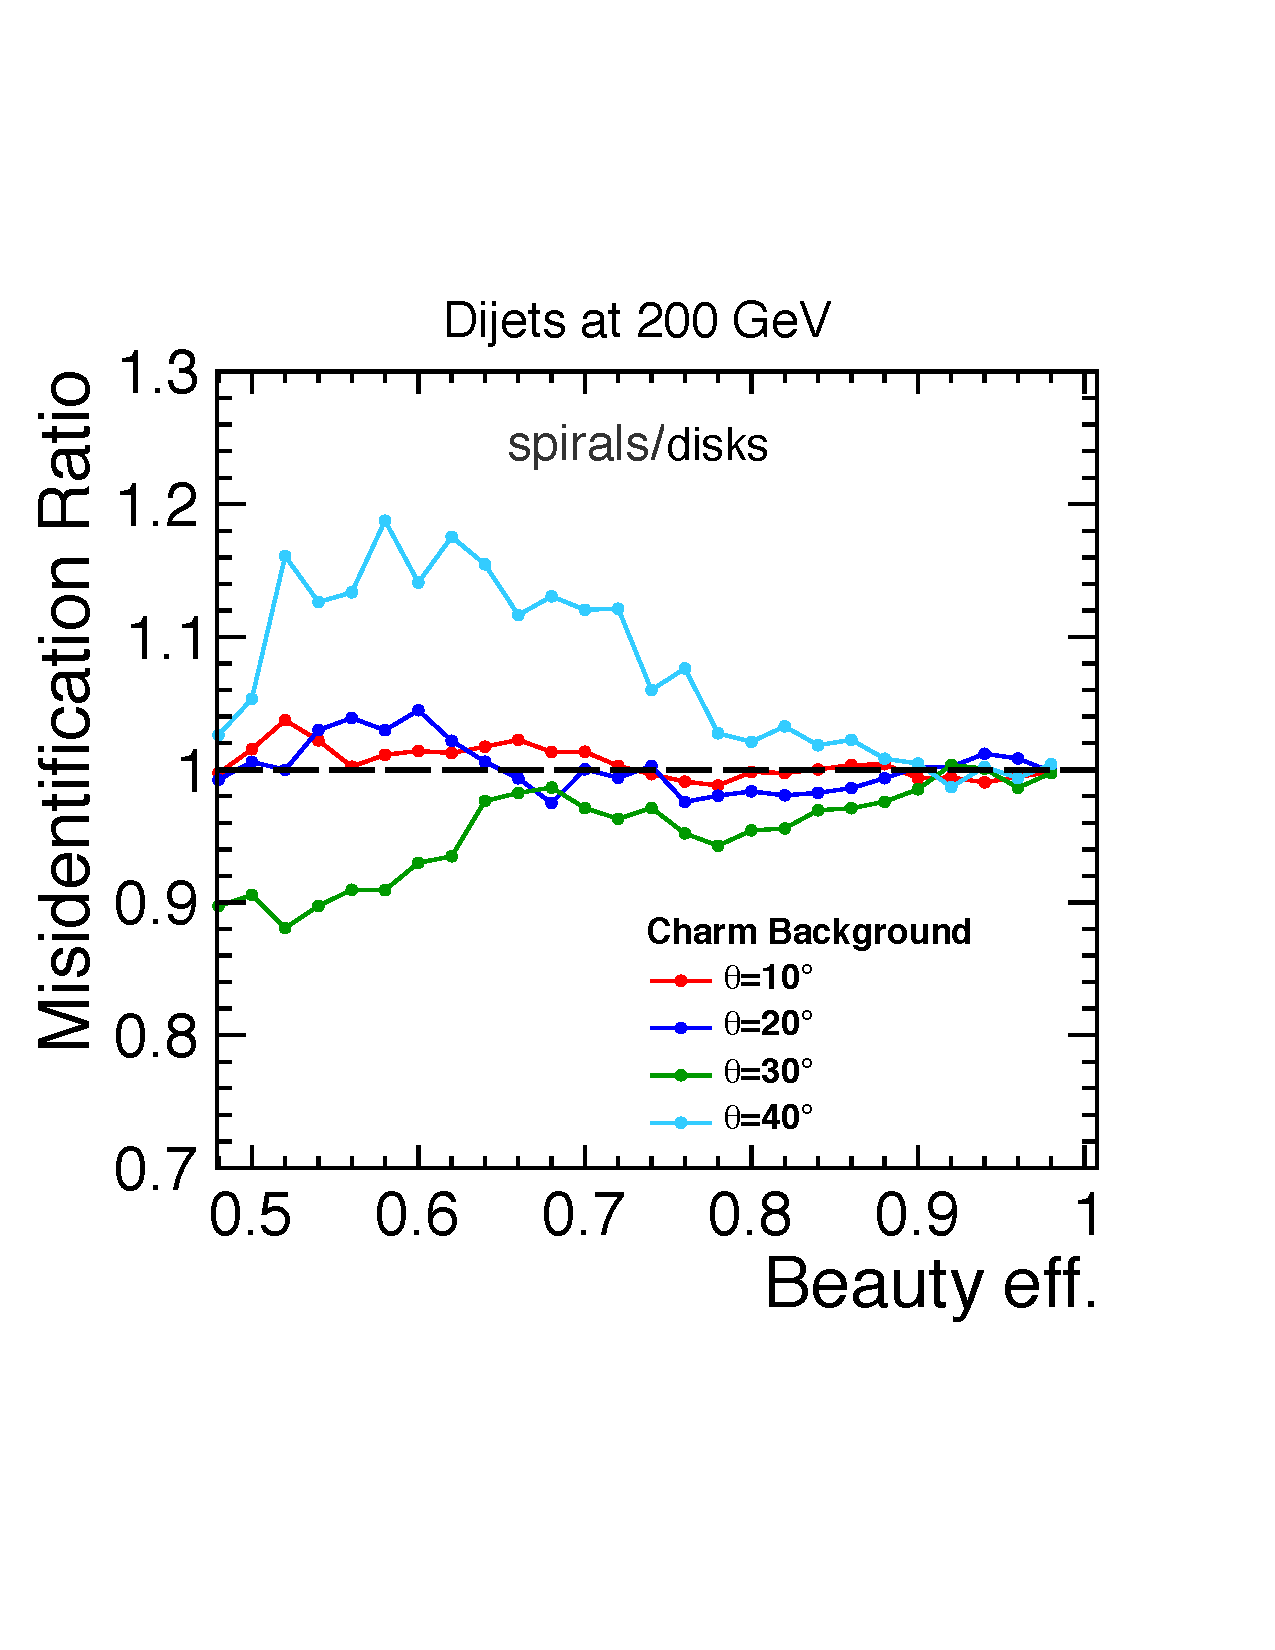
\includegraphics[trim = 5mm 50mm 20mm 20mm, clip, width=\textwidth]{figures/CLIC/200GeV_Ratio_allAngles_spirals_CDR_B_C.pdf}};
      \draw  (1.8, 1.5) node {\textbf{CLICdp}};
    \end{tikzpicture}
    \caption{}
    \label{fig:spiral_disks}
  \end{subfigure}~
  \begin{subfigure}[b]{0.33\textwidth}
    \centering
    \begin{tikzpicture}
      \node[anchor=south west, inner sep=0] (image) at (0,0){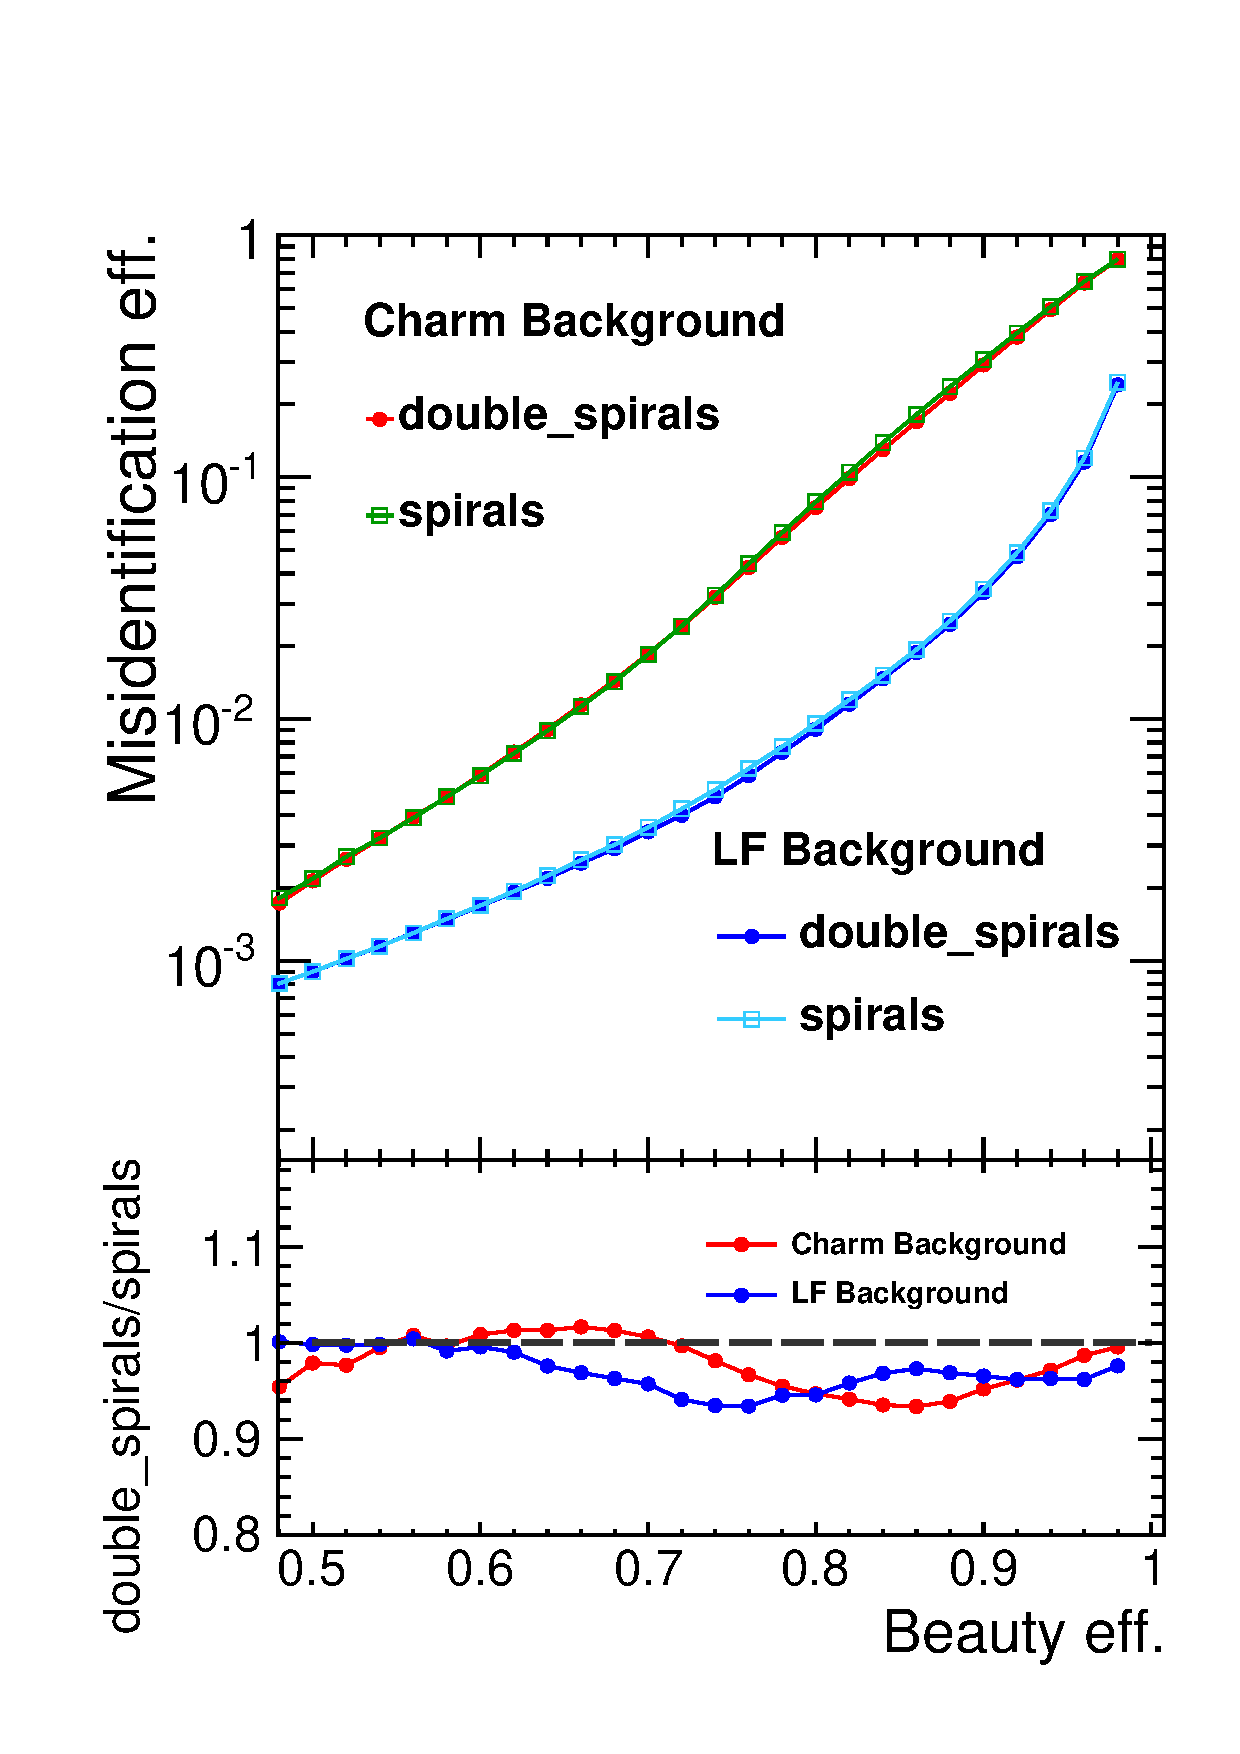
\includegraphics[width=\textwidth]{figures/CLIC/general_200_Beauty.pdf}};
      \draw (1.8, 2.8) node {\textbf{CLICdp}};
    \end{tikzpicture}
    \caption{}
    \label{fig:spiral_doubleSpirals}
  \end{subfigure}~
  \begin{subfigure}[b]{0.33\textwidth}
    \centering
    \begin{tikzpicture}
      \node[anchor=south west, inner sep=0] (image) at (0,0){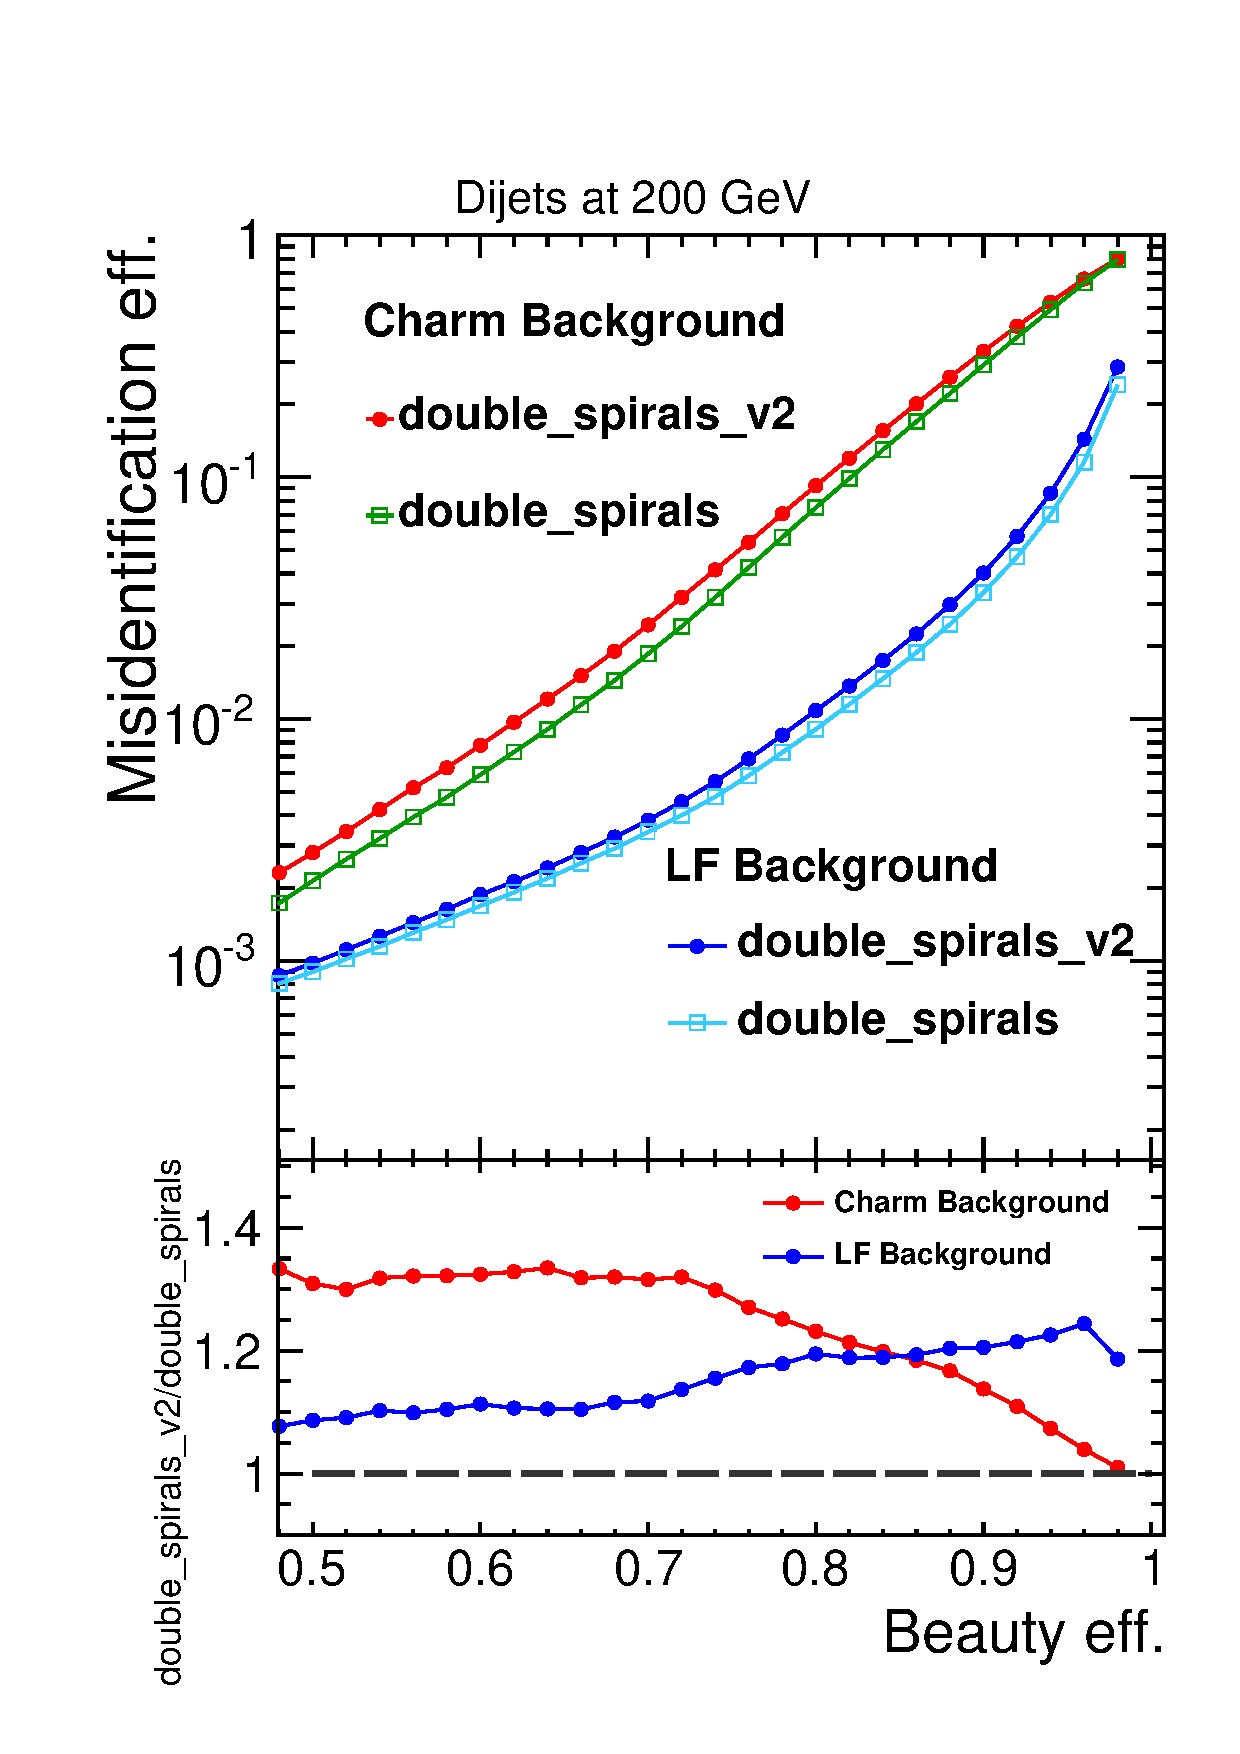
\includegraphics[width=\textwidth]{figures/CLIC/heavy_general_200_Beauty.pdf}};
      \draw (1.8, 2.8) node {\textbf{CLICdp}};
    \end{tikzpicture}
    \caption{}
    \label{fig:doubleSpirals_doubleSpirals}
  \end{subfigure}
  \caption{Beauty-tagging performance for dijet events at
    \SI{200}{\giga\electronvolt}. (a)~Comparison between \emph{disks}
    and \emph{spirals} in terms of the ratio of the misidentification
    probabilities for charm background. (b)~Comparison of the
    beauty-tagging performance between the \emph{spirals} and
    \emph{double\_spirals} geometries. (c)~Comparison of the
    beauty-tagging performance between the \emph{double\_spirals} and
    \emph{double\_spirals\_v2} geometries. For (a) the
    misidentification ration for each polar angle is shown
    separately. For (b) and (c), dijet events with a mixture of polar
    angles between \SI{10}{\degree} and \SI{90}{\degree} are
    considered.}
  \label{fig:performance}
\end{figure}

The CLIC detector model for simulations is under development with the
requirements set by the precision physics to be measured. With these
requirements, it allows for identification of beauty and charm quarks
and this is possible with a vertex detector with a high spatial
resolution and very low material budget to limit the multiple
scatterings. This thesis focuses on the R\&D of the pixel detectors in
the vertex detector with high-resolution and very low material budget.

% ============================================================================== 
% planning for the chapter
% ============================================================================== 
% Accelerator (two-beam acceleration), CLIC detector concept, picture of
% the full detector (3 pages)

% \section{Requirements for the CLIC vertex detector}
% motivation for pixel detectors in high-energy physics (flavour-tagging
% plots), requirements, design, technical challenges
% (cooling/mechanics), Beam induced backgrounds, Radiation damage in the
% vertex detector (3 pages).


% \section{Flavour tagging at CLIC}
% say motivation of this thesis $\Rightarrow$ provide input for the
% digitiser (1 page) and the detector simulation software.
